\documentclass[a4paper,twocolumn,10pt]{ltjsarticle}
\usepackage{luatexja-fontspec}
\setmainfont{TeX Gyre Termes}
\setmainjfont{Noto Serif CJK JP}
\setsansjfont{Noto Sans CJK JP}
\usepackage{amsmath,amssymb,bm}
\usepackage{graphicx}
\usepackage{rotating}
\usepackage{booktabs}
\usepackage{siunitx}
\usepackage[margin=17mm,columnsep=7mm]{geometry}
\usepackage{caption}
\captionsetup{font=small,labelsep=quad}
\usepackage[hidelinks]{hyperref}
\usepackage{enumitem}
\setlist{nosep,leftmargin=1.4em}
\graphicspath{{../figures/}{../../results/}{../../media/}}
\renewcommand{\figurename}{図}
\renewcommand{\tablename}{表}

\title{\vspace{-6mm}\textbf{SoftTwin：学習アクチュエータモデル・固有感覚・布状触覚スキンで\\「触って確かめてからつかむ」空圧ソフトグリッパと\\自動アノテーション触覚データ生成}}
\author{isobe\_97\quad（Physical AI 講座 2026 応用編1 最終課題）}
\date{}

\begin{document}
\twocolumn[
\maketitle
\vspace{-8mm}
\begin{center}
\begin{minipage}{0.92\textwidth}
\small
\textbf{概要}\quad
食品工場や物流の現場では，いちご・豆腐・卵のように壊れやすさが大きく異なる物体を，同じハンドで扱うことが求められる．
空圧ソフトグリッパは柔らかい物の把持に向くが，内圧を固定する一般的な運用では，壊れやすい物を潰すか，重い物を落とすかのどちらかになりやすい．
本研究では，(1) 内圧から自由曲げ角を予測する学習アクチュエータモデル，(2) 指のたわみから把持力を推定する固有感覚推定器，
(3) 言語指示から目標把持力を決める VLM タスク計画器，(4) 指の内側に貼る布状触覚スキン（24 点）と，0.4\,N だけ触って硬さを測り目標把持力を決め直す「触覚プローブ」，
(5) 画像・深度・マスク・触覚・内圧・関節角・真の接触力・成否を\textbf{人手なしで自動アノテーション}するデータ生成器，を組み合わせた SoftTwin を設計・実装した．
MuJoCo 上で質量・摩擦・表面の柔らかさをランダム化した 5 物体 × 10 シードの評価で，提案の力制御は成功率 96\,\%・破損率 0\,\% を達成し，
内圧固定（20\,kPa：78\,\%／20\,\%，60\,kPa：60\,\%／40\,\%）と線形アクチュエータモデルの閉ループ（70\,\%，落下 30\,\%）を上回った．
さらに，見た目は同じで中身が違う物体（完熟トマト・樹脂の食品サンプル）を加えた 7 物体では，VLM の事前知識だけだと成功 76\,\%・破損 14\,\%（見た目が同じ物体では成功 25\,\%）だったのに対し，
420 試行・4.6 分で自動生成したデータで学習した画像＋触覚の分類器を使うと成功 91\,\%・破損 4\,\%（同 90\,\%）となり，真値クラスを与えた上限（93\,\%）に近づいた．
実機の人工筋肉と触覚スキンは仮定したモデルで代替しており，実機での検証は今後の課題である．
\end{minipage}
\end{center}
\vspace{4mm}
]

\section{はじめに}
ソフトロボットハンドは，シリコーンなどの柔軟材料の変形を利用して対象に倣うため，食品のように形状や硬さがばらつく物体の把持に適している\cite{shintake2018}．
特に空気圧で曲がる PneuNet 型アクチュエータ\cite{ilievski2011,mosadegh2014}は構造が単純で安価に作れる．一方で，
\begin{itemize}
\item 曲げ角が内圧に対して非線形で，不感帯・遅れ・ヒステリシスを持つため，物理シミュレータで再現しにくい（sim-to-real の差が大きい），
\item 力センサを指に埋め込むと柔らかさやコストが損なわれるため，把持力を直接測れない，
\item 物体ごとに許容できる力が 1\,N 程度から数十 N まで大きく異なるため，内圧を固定する運用では破損と落下を両立して防げない，
\end{itemize}
という課題がある．本研究の貢献は次の 4 点である．
\begin{enumerate}
\item 入力と出力を明示したシステム構成（図\ref{fig:block}）にもとづく，実機・デジタルツイン・アプリ層を分離したアーキテクチャの設計．
\item 内圧の時系列から自由曲げ角を予測する小規模 MLP（学習アクチュエータモデル）．線形モデルに比べ曲げ角誤差を 85\,\% 低減した．
\item 疑似剛体モデル（PRBM）\cite{howell2001}の関節たわみから指先力を最小二乗推定する，追加センサ不要の固有感覚把持力推定器．
\item 言語指示から決まる目標把持力に，接触検知時の指令リセットと比例制御で追従する力制御器と，落下時の再把持．
\item 布状触覚スキンのセンサモデルと触覚プローブ．カメラでは見えない「柔らかさ」を 0.4\,N の押し込みで測り，VLM の事前知識を上書きする．
\item 画像と触覚・圧力を同時に自動アノテーションするデータ生成器．ピッキング現場で課題になる「触覚付きの学習データを量産できない」問題に，シミュレーションで答える．
\end{enumerate}

\begin{sidewaysfigure*}
\centering
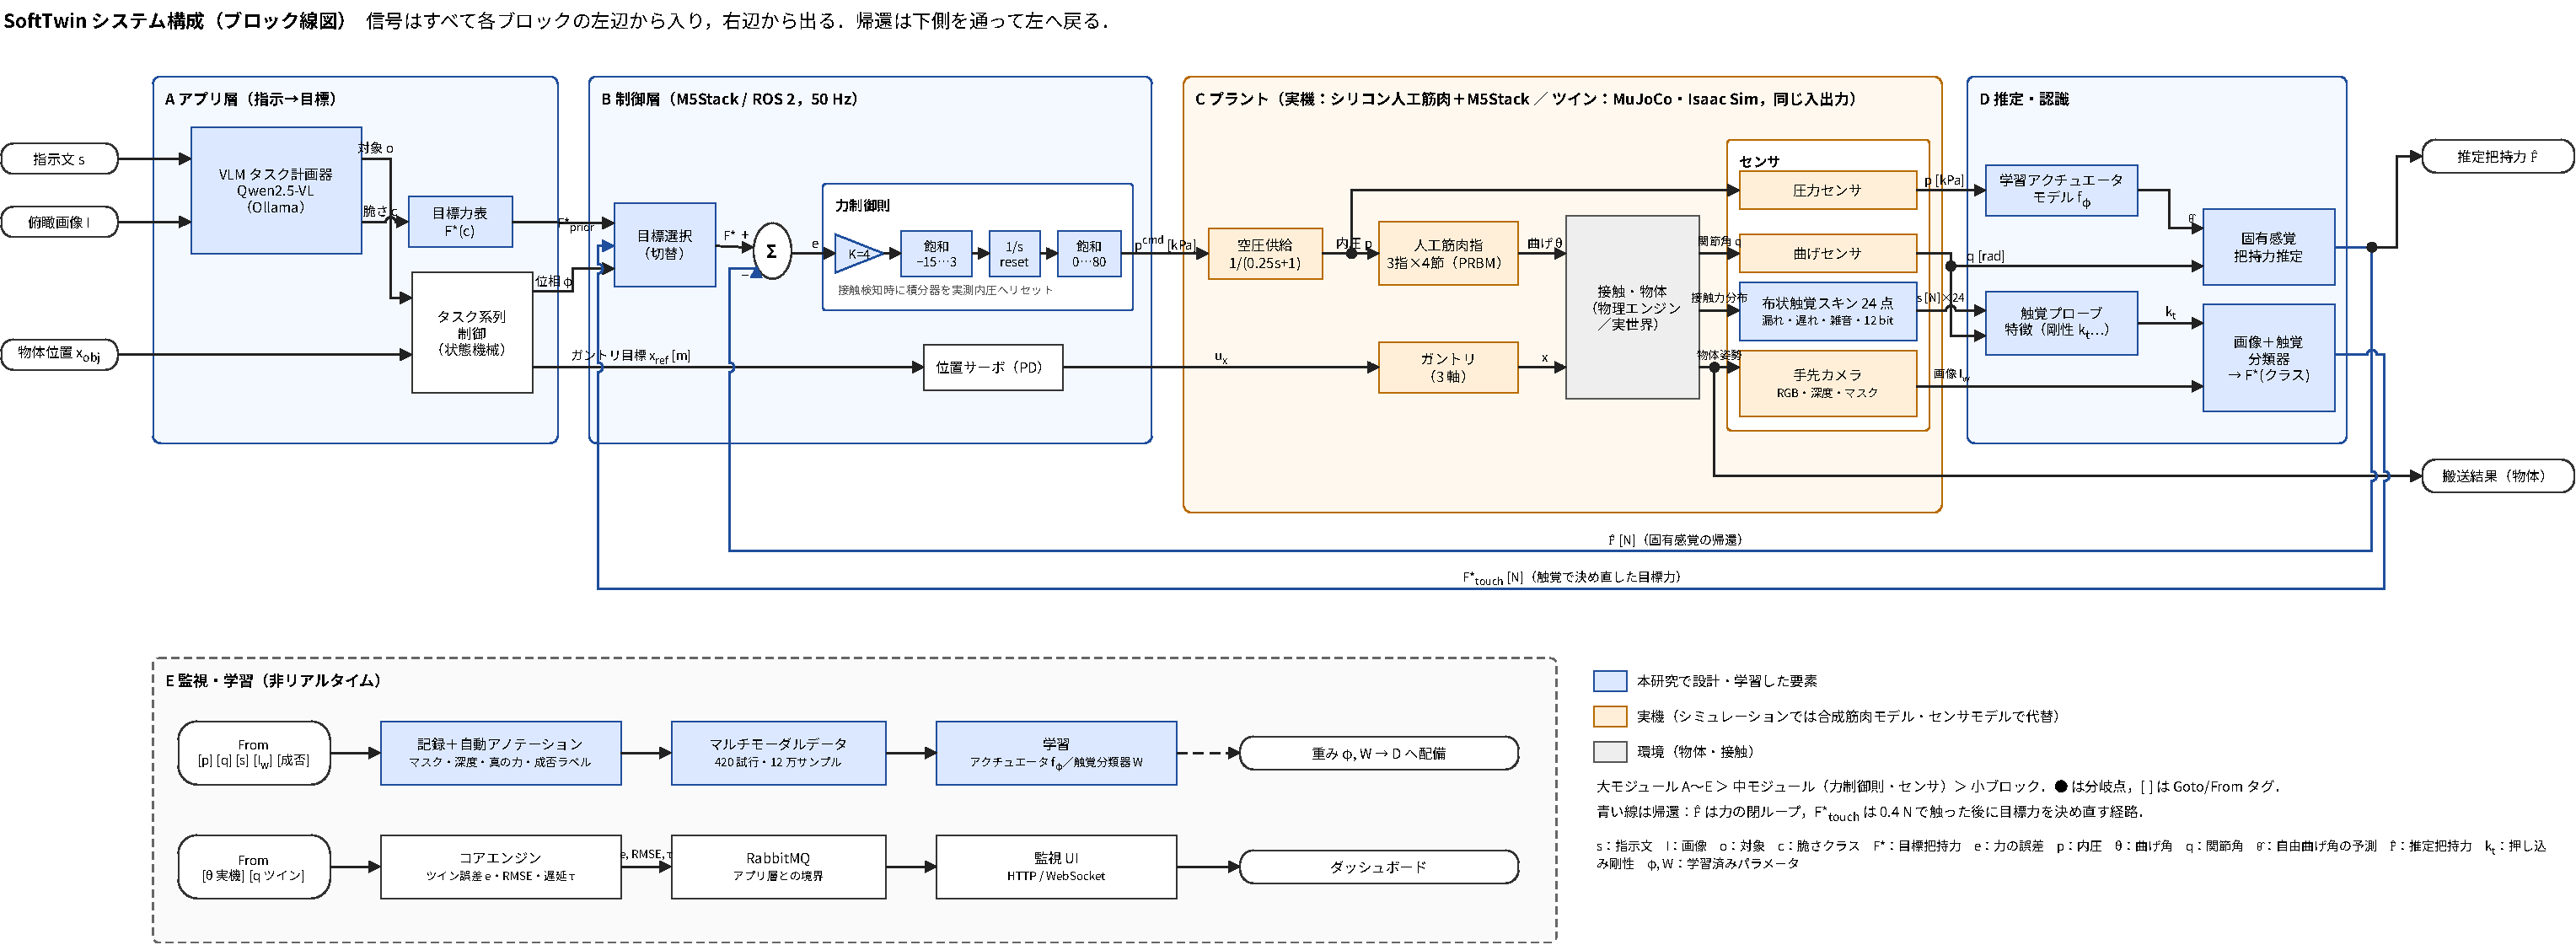
\includegraphics[width=\textheight]{block_diagram.pdf}
\caption{SoftTwin のシステム構成（ブロック線図，draw.io）．すべてのブロックは左辺から入力を受け右辺へ出力し，信号は左上から右下へ流れる．帰還（青線）は下側を通って左へ戻る．
大モジュール A（アプリ層）→ B（制御層）→ C（プラント：実機またはツイン，同じ入出力）→ D（推定・認識）が実時間ループを作り，E（監視・学習）は非実時間で重みを更新する．
青は本研究で設計・学習した要素，橙は実機（シミュレーションでは合成筋肉モデル・センサモデルで代替）．}
\label{fig:block}
\end{sidewaysfigure*}

\section{システム構成}
目的を「壊れやすさの異なる物体を，指示どおりに，潰さず落とさず搬送する」と定め，評価指標を成功率・破損率・落下率，ツインの曲げ角誤差，制御ループ遅延とした．
そこから逆算して必要な信号を表\ref{tab:io}のように定義した．
実機では M5Stack（ESP32）がポンプと電磁弁で内圧を制御し，圧力 $p$ と曲げ角 $\theta$ を micro-ROS で 50\,Hz 配信する．
シミュレータ（Isaac Sim / MuJoCo）は同じ $p$ を学習アクチュエータモデルに通して関節目標を作り，実機と同じ指令で動くデジタルツインになる．
コアエンジンは実機とツインの差 $e$，誤差の RMSE，ループ遅延 $\tau$ を計測し，RabbitMQ 経由でアプリ層と監視 UI に配信する．
記録はオフラインで LeRobot 形式に変換し，アクチュエータモデルの再学習に用いる．

\begin{table}[t]
\centering\small
\caption{主要ブロックの入力と出力}
\label{tab:io}
\begin{tabular}{@{}p{22mm}p{24mm}p{25mm}@{}}
\toprule
ブロック & 入力 & 出力 \\
\midrule
VLM 計画器 & 指示文 $s$，画像 $I$ & 対象 $o$，脆さ $c$ \\
タスク系列制御 & $o,c$，物体位置 & ガントリ目標 $\mathbf{x}^{\rm ref}$，$F^*(c)$ \\
把持力制御器 & $F^*$，推定 $\hat F$ & 内圧指令 $p^{\rm cmd}$ [kPa] \\
空圧供給 & $p^{\rm cmd}$ & 内圧 $p$ [kPa] \\
アクチュエータ & $p,\dot p,\hat\theta_{k-1}$ & 自由曲げ角 $\hat\theta$ [deg] \\
ツイン (PRBM) & $\theta^{\rm ref}=\hat\theta/N$ & 関節角 $\mathbf q$，物体姿勢 \\
力推定器 & $\theta^{\rm ref}$，$\mathbf q$ & 推定把持力 $\hat F$ [N] \\
コアエンジン & $\theta$（実機），$\mathbf q$ & $e$，RMSE，遅延 $\tau$ \\
\bottomrule
\end{tabular}
\end{table}

\section{手法}
\subsection{疑似剛体モデルによる柔軟指}
各指（3 本，120° 間隔）を長さ $L=26$\,mm の剛体セグメント $N=4$ 個と回転関節で近似した．
関節は位置サーボ（剛性 $k_b=0.5$\,N\,m/rad，減衰 $d_b=0.006$）で表し，目標角 $\theta^{\rm ref}=\hat\theta/N$ をシリコーンの自由曲げとして与える．
接触があると関節が目標から遅れてたわむため，受動的な倣いが再現される．

\subsection{学習アクチュエータモデル}
内圧 $p$ から自由曲げ角 $\hat\theta$ への写像を，入力 $[p_k,\dot p_k,\hat\theta_{k-1}]$，隠れ層 48×2（tanh）の MLP で表した．
学習は 1 ステップ先予測（教師強制）で行い，評価は自身の出力だけを使う自己回帰ロールアウトで行う．
データは軌道（ステップ・ランプ・正弦）単位で学習用と評価用に分け，リークを防いだ．
実機データが揃うまでは，不感帯 6\,kPa・飽和型の静特性・時定数 0.12\,s の遅れ・方向依存ヒステリシス 6° を持つ合成筋肉モデルで代替した．
Hwangbo らのアクチュエータネット\cite{hwangbo2019}と同じく，解析モデル化が難しいアクチュエータを学習で埋める考え方である．

\subsection{固有感覚による把持力推定}
指先で力 $F$ を受けると，関節 $j$ には $\tau_j \approx F\,l_j$（$l_j=(N-j)L$）のトルクがかかる．
関節トルクは目標とのずれから $\tau_j = k_b(\theta^{\rm ref}_j-q_j) - d_b\dot q_j$ と求まるので，指ごとに最小二乗で
\begin{equation}
\hat F_f = \frac{\sum_j \tau_j l_j}{\sum_j l_j^2},\qquad \hat F=\sum_f \max(\hat F_f,0)
\end{equation}
とした．実機では $\theta^{\rm ref}$ に学習モデルの予測を，$q$ に曲げセンサの値を用いるため，推定精度はアクチュエータモデルの精度で決まる．

\subsection{力制御器とタスク計画}
VLM 計画器（Qwen2.5-VL\cite{qwen25vl}，Ollama 経由）は指示文と俯瞰画像から対象と脆さクラス $c$ を出力し，
$F^*$ を very\_fragile 0.7\,N，fragile 1.8\,N，rigid 3.5\,N に設定する．
把持力制御器は，接触前は 12\,kPa/s で加圧し，$\hat F \ge 0.15F^*$ で接触を検知した時点で指令を現在の内圧にリセットして供給系の遅れによる行き過ぎを防ぐ．
以後は $\dot p^{\rm cmd} = \mathrm{clip}(4(F^*-\hat F), -15, 3)$\,kPa/s で追従し，搬送中も同じ制御を続けて加速度による荷重変化に対応する．
持ち上げ後に物体が卓上に残った場合は，$F^*$ を 1.4 倍（許容力の 70\,\% まで）にして最大 2 回再把持する．

\subsection{布状触覚スキンと触覚プローブ}
指の各セグメントの内側に，布状の感圧センサを 2 枚ずつ（根元側・指先側）貼ることを想定し，計 24 点のタクセル $\mathbf s$ とした．
シミュレータの接触力をそのまま使わず，実在の布状センサに近づけるため，隣接タクセルへのクロストーク 10\,\%，個体ごとの感度誤差 8\,\%，
時定数 15\,ms の遅れ，ノイズ 6\,mN，不感帯 20\,mN，8\,N で飽和，12\,bit の量子化を加えたセンサモデルを通した（いずれも仮定値）．
把持では，まずスキンの合計が 0.08\,N を超えた時点を接触とし（アクチュエータモデルの誤差に左右されない），$F^*=0.4$\,N まで弱く握る．
このとき指ごとに「スキンの力の増分 ÷ その指の追加の曲げ角」を押し込み剛性 $k_{\rm t}$ [N/deg] として求め，内圧・接触面積・荷重位置など計 10 個の特徴量にまとめる．
手先カメラ画像からは物体の平均色・面積・縦横比の 5 個を取り，両者を多クラスロジスティック回帰に入れて扱い方クラス（極脆・軟・脆・剛）を推定し，$F^*$ を決め直す．

\subsection{自動アノテーション付きデータ生成}
物体の柔らかさは MuJoCo の接触パラメータ（solref の時定数と solimp）で表し，見た目は同じで中身が違う 2 物体（完熟トマト：軟らかく許容 1.5\,N，食品サンプル：硬く重く滑りやすい）を加えた．
各試行で物体・配置・質量・摩擦・柔らかさをランダム化し，プローブの後の目標把持力も 0.5--4.0\,N から無作為に選ぶ．こうすると成功だけでなく破損や滑落の例も自然に集まる．
1 試行ごとに，手先カメラの RGB・深度・セグメンテーションマスク・バウンディングボックス，50\,Hz の内圧・関節角・推定把持力・真の接触力・スキン 24 点（センサモデル後と真値），
物体名・見た目の物体・真のクラス・隠れた物理量・成否（成功／破損／滑落）をすべてシミュレータから自動で書き出す（表\ref{tab:ds}）．

\begin{table}[t]
\centering\small
\caption{自動生成したデータセット（人手のアノテーションなし）}
\label{tab:ds}
\begin{tabular}{@{}p{20mm}p{50mm}@{}}
\toprule
規模 & 420 試行（7 物体 × 60），2 CPU で 4.6 分 \\
時系列 & 12 万サンプル（50\,Hz）：$p^{\rm cmd}, p, \hat\theta, \mathbf q, \hat F, F, \mathbf s, \mathbf s^{\rm true}$ \\
画像 & 手先 RGB・深度・マスク，全体 RGB・マスク（把持中・持ち上げ後） \\
ラベル & 物体，見た目，真のクラス，質量・摩擦・柔らかさ，目標力，成功 55\,\%／破損 24\,\%／滑落 21\,\% \\
形式 & \texttt{index.parquet}／\texttt{jsonl}，試行ごとの \texttt{npz} \\
\bottomrule
\end{tabular}
\end{table}

\section{実験}
\subsection{条件}
MuJoCo~3.15\cite{todorov2012}（時間刻み 1\,ms，制御 50\,Hz）で，テーブル・3 軸ガントリ・3 本指グリッパ・トレーからなるセルを構築した．
物体 5 種（表\ref{tab:obj}）を 10 シードで配置し，質量 ±25\,\%，摩擦 ±20\,\%，表面の柔らかさ ±15\,\% をランダム化した．
許容力は文献値ではなく本実験の仮定値である．
実機の代わりに合成筋肉モデルが指を駆動し，制御器は学習（または線形）モデルの予測だけを知る条件で評価した．
破損は接触力の真値（20\,ms 移動平均）が許容力を超えた場合，成功は破損も落下もなくトレーに置けた場合とした．

\begin{table}[t]
\centering\small
\caption{評価物体（許容力は本実験の仮定値，$^\dagger$：見た目がトマト／いちごと同じ）}
\label{tab:obj}
\begin{tabular}{@{}lrrll@{}}
\toprule
物体 & 質量 [g] & 許容力 [N] & クラス & $F^*$ [N] \\
\midrule
いちご & 18 & 3.0 & fragile & 1.8 \\
卵 & 60 & 25.0 & fragile & 1.8 \\
豆腐 & 35 & 1.2 & very\_fragile & 0.7 \\
トマト & 90 & 10.0 & fragile & 1.8 \\
ボルト & 35 & -- & rigid & 3.5 \\
\midrule
完熟トマト$^\dagger$ & 90 & 1.5 & soft & 1.3 \\
食品サンプル$^\dagger$ & 40 & -- & rigid & 3.5 \\
\bottomrule
\end{tabular}
\end{table}

\subsection{結果}
\textbf{アクチュエータ同定．}評価用 16 軌道の自己回帰ロールアウトで，曲げ角 RMSE は線形モデル 14.8° に対し学習モデル 2.2°（85\,\% 減）となった（図\ref{fig:fit}）．
\textbf{把持・搬送．}表\ref{tab:res}・図\ref{fig:bench}に示すとおり，内圧固定は 20\,kPa で豆腐を，60\,kPa ではいちごと豆腐を潰した．
線形モデルの閉ループは破損 0\,\% だが落下が 30\,\% あり，豆腐は全数落下した．
提案法は成功率 96\,\%，破損 0\,\%，平均試行回数 1.04 だった．
\textbf{力推定．}推定と真値の平均絶対誤差は，提案法 0.17\,N，線形モデル 0.40\,N だった．
図\ref{fig:force}のとおり，線形モデルは自由曲げを過大に見積もるため，指が触れていない段階で「目標の力に達した」と誤認し，把持が成立しない．

\begin{table}[t]
\centering\small
\caption{把持・搬送の結果（各手法 50 試行）}
\label{tab:res}
\begin{tabular}{@{}lrrrr@{}}
\toprule
手法 & 成功 & 破損 & 落下 & 推定誤差 \\
\midrule
開ループ 20\,kPa & 78\,\% & 20\,\% & 2\,\% & 0.29\,N \\
開ループ 60\,kPa & 60\,\% & 40\,\% & 0\,\% & 0.62\,N \\
閉ループ（線形） & 70\,\% & 0\,\% & 30\,\% & 0.40\,N \\
\textbf{閉ループ（提案）} & \textbf{96\,\%} & \textbf{0\,\%} & 2\,\% & \textbf{0.17\,N} \\
\bottomrule
\end{tabular}
\end{table}

\subsection{触覚：見た目が同じ物体の見分けと把持}
\textbf{分類．}自動生成データを試行単位で 7:3 に分けると（学習 294，評価 126），扱い方クラスの正解率は画像のみ 67\,\%，触覚のみ 96\,\%，画像＋触覚 98\,\% だった（図\ref{fig:tactile}d）．
画像のみではトマトと完熟トマト，いちごと食品サンプルを区別できない．押し込み剛性の中央値は，トマト 0.10 に対し完熟トマト 0.037，いちご 0.054 に対し食品サンプル 0.11\,N/deg と明確に分かれた（図\ref{fig:tactile}c）．
成否ラベルを目標力ごとに集計すると，クラスごとに「落とさず潰さない力の窓」が現れ（図\ref{fig:tactile}e），軟クラスでは窓が 1.0--1.5\,N と狭い．
\textbf{閉ループ評価．}7 物体 × 10 シード（データ生成とは別のシード）で，学習済み分類器をオンラインで使って比較した（表\ref{tab:la}，図\ref{fig:la}）．
VLM の事前知識だけでは完熟トマトを「トマト＝1.8\,N」で握って全数潰し，食品サンプルを「いちご＝1.8\,N」で握って半数を落とした．
画像＋触覚では見た目が同じ物体の成功率が 25\,\% から 90\,\% に上がった．代償はプローブにかかる約 2.2\,s のサイクルタイム増である．

\begin{table}[t]
\centering\small
\caption{見た目が同じ物体を含む 7 物体の結果（各 70 試行）}
\label{tab:la}
\begin{tabular}{@{}lrrrr@{}}
\toprule
$F^*$ の決め方 & 成功 & 破損 & 同形物体 & 時間 \\
\midrule
VLM 事前知識のみ & 76\,\% & 14\,\% & 25\,\% & 11.7\,s \\
画像分類器 & 74\,\% & 19\,\% & 65\,\% & 14.6\,s \\
触覚分類器 & 87\,\% & 4\,\% & 80\,\% & 14.5\,s \\
\textbf{画像＋触覚（提案）} & \textbf{91\,\%} & \textbf{4\,\%} & \textbf{90\,\%} & 13.9\,s \\
真値クラス（上限） & 93\,\% & 3\,\% & 85\,\% & 11.2\,s \\
\bottomrule
\end{tabular}
\end{table}

\begin{figure*}[t]
\centering
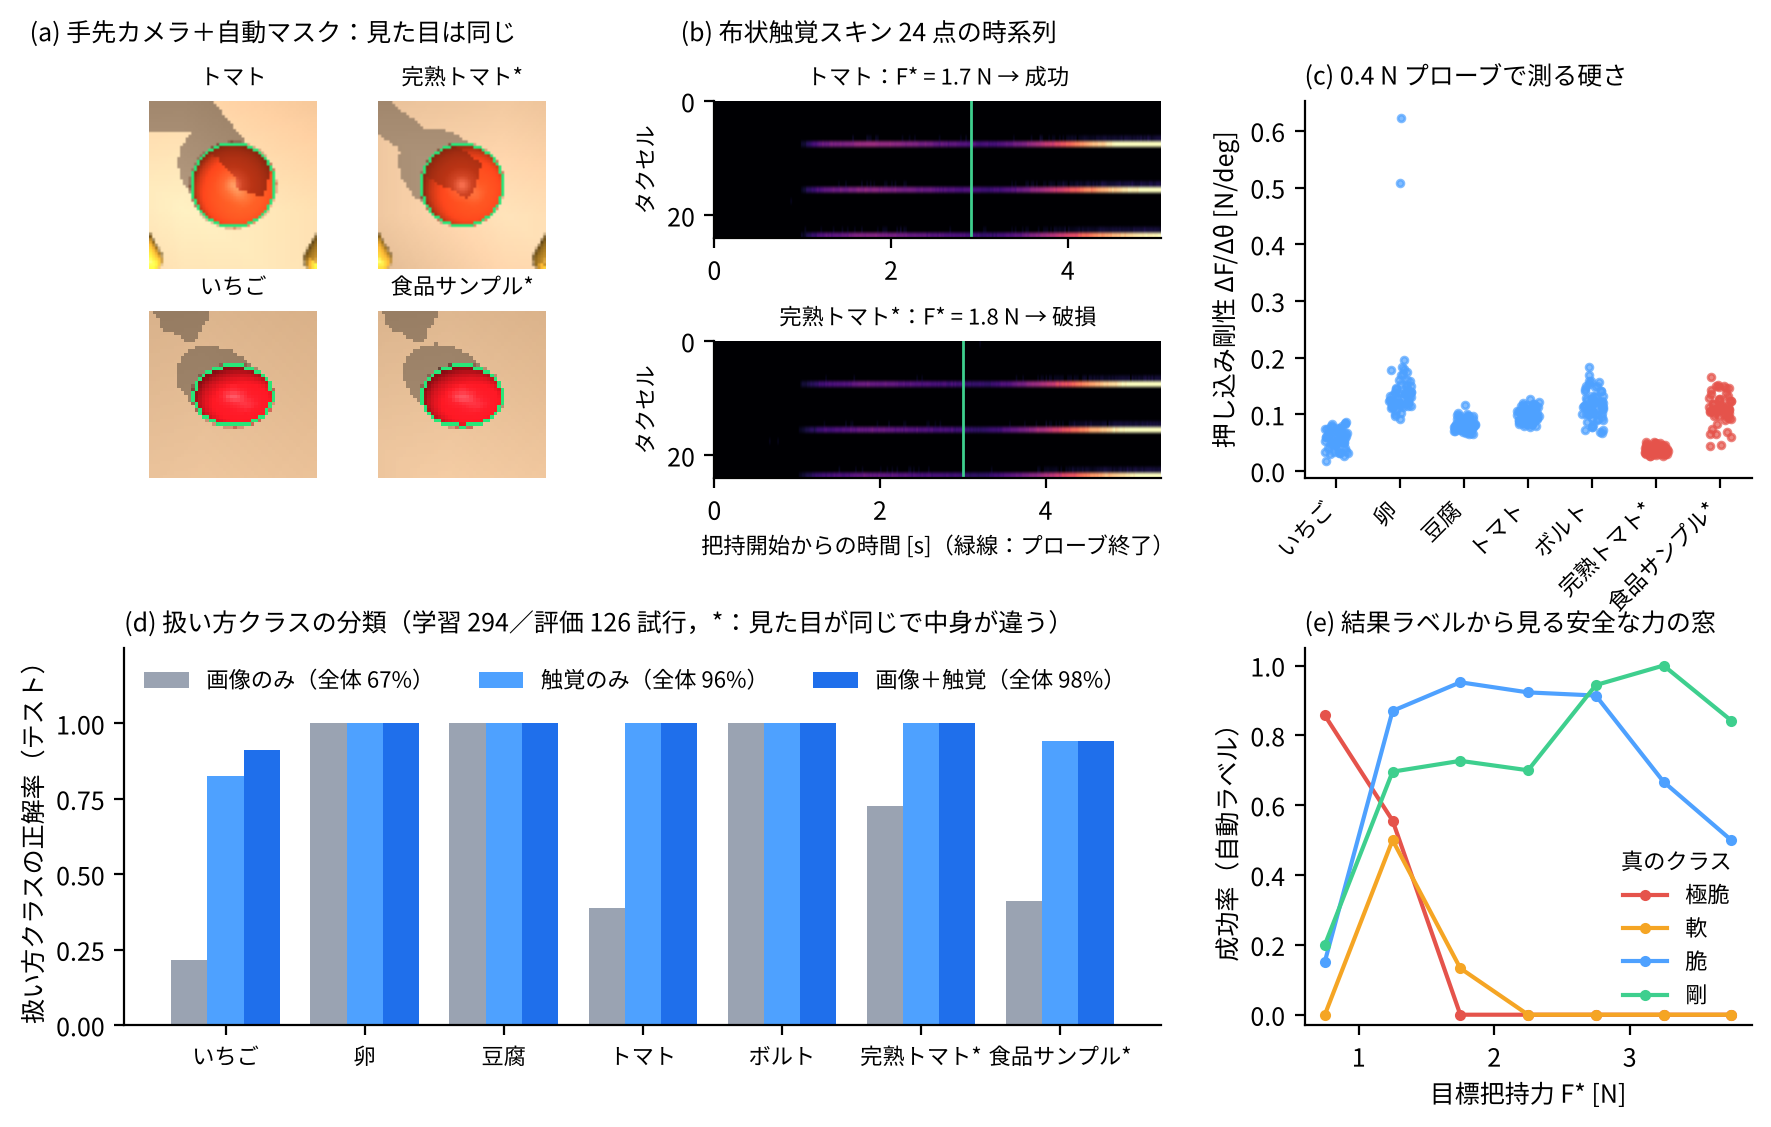
\includegraphics[width=0.96\textwidth]{fig_tactile.png}
\caption{触覚スキンと自動アノテーションデータ．(a) 手先カメラ画像と自動生成マスク（緑）．(b) 同じ目標力で握ったトマトと完熟トマトのスキン 24 点の時系列．
(c) 0.4\,N プローブで測った押し込み剛性（赤：見た目が同じで中身が違う物体）．(d) 扱い方クラスの分類正解率．(e) 成否ラベルから求めたクラス別の成功率と目標把持力．}
\label{fig:tactile}
\end{figure*}

\begin{figure}[t]
\centering
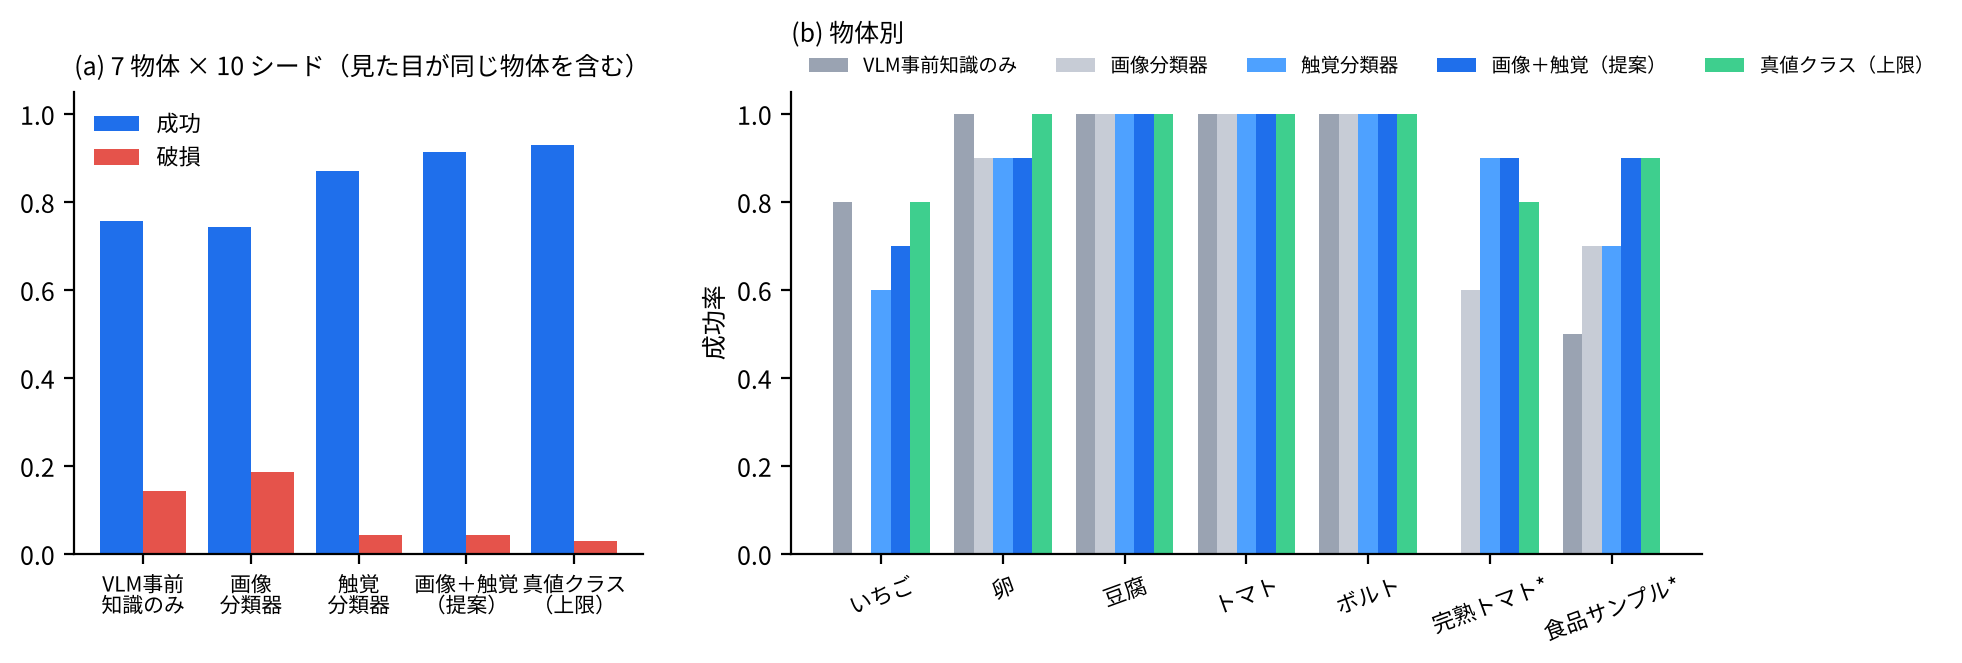
\includegraphics[width=\columnwidth]{fig_lookalike.png}
\caption{見た目が同じ物体を含む閉ループ評価．}
\label{fig:la}
\end{figure}

\begin{figure}[t]
\centering
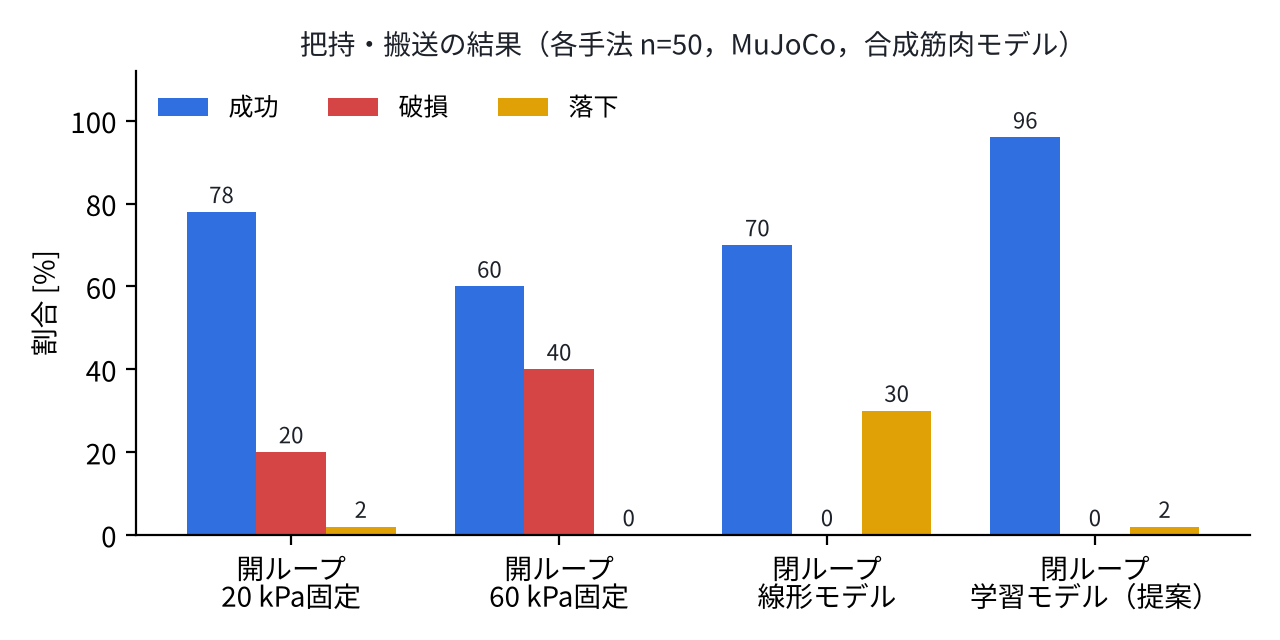
\includegraphics[width=\columnwidth]{fig_benchmark.png}
\caption{手法ごとの成功・破損・落下の割合．}
\label{fig:bench}
\end{figure}

\begin{figure}[t]
\centering
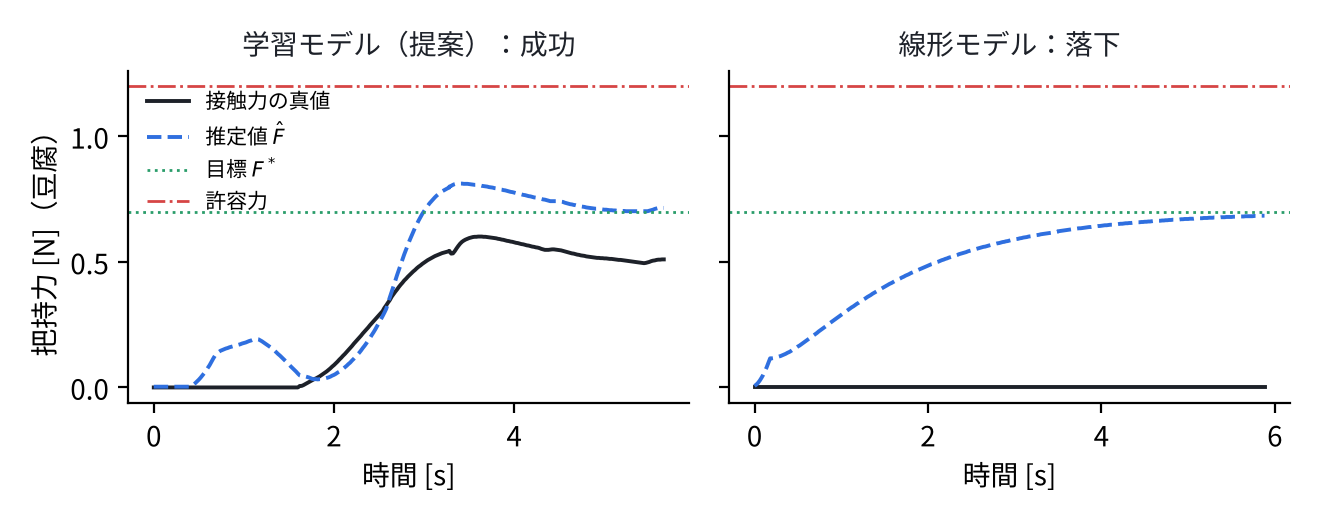
\includegraphics[width=\columnwidth]{fig_force_tracking.png}
\caption{豆腐を把持したときの推定把持力と接触力の真値．線形モデルは接触前に目標到達と誤認する．}
\label{fig:force}
\end{figure}

\begin{figure}[t]
\centering
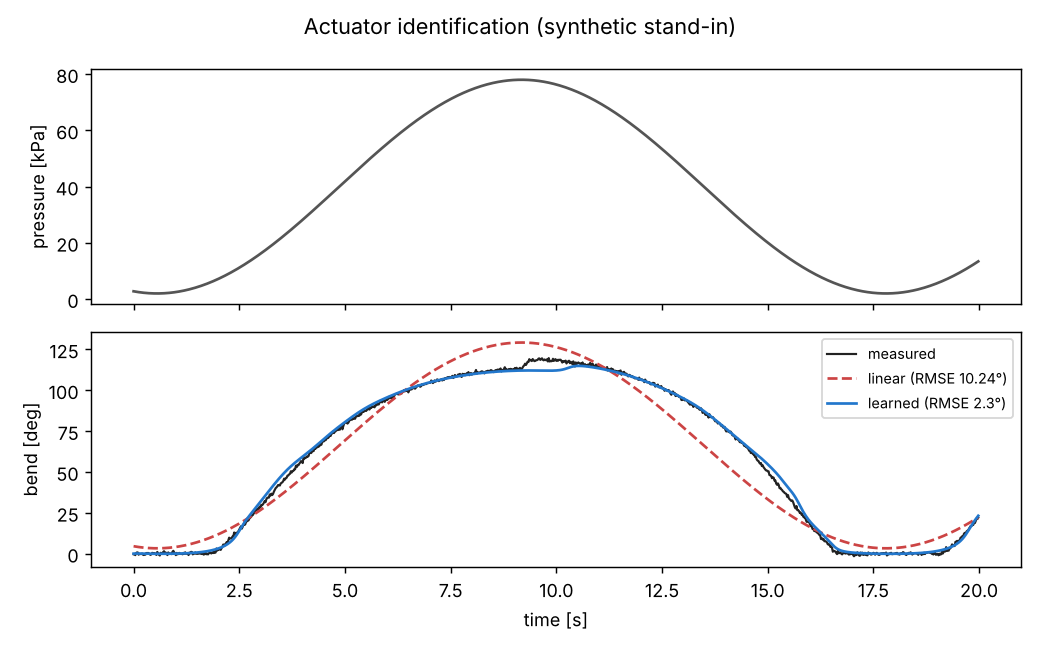
\includegraphics[width=\columnwidth]{actuator_fit.png}
\caption{アクチュエータ同定の例（合成データ，評価用軌道）．}
\label{fig:fit}
\end{figure}

\begin{figure}[t]
\centering
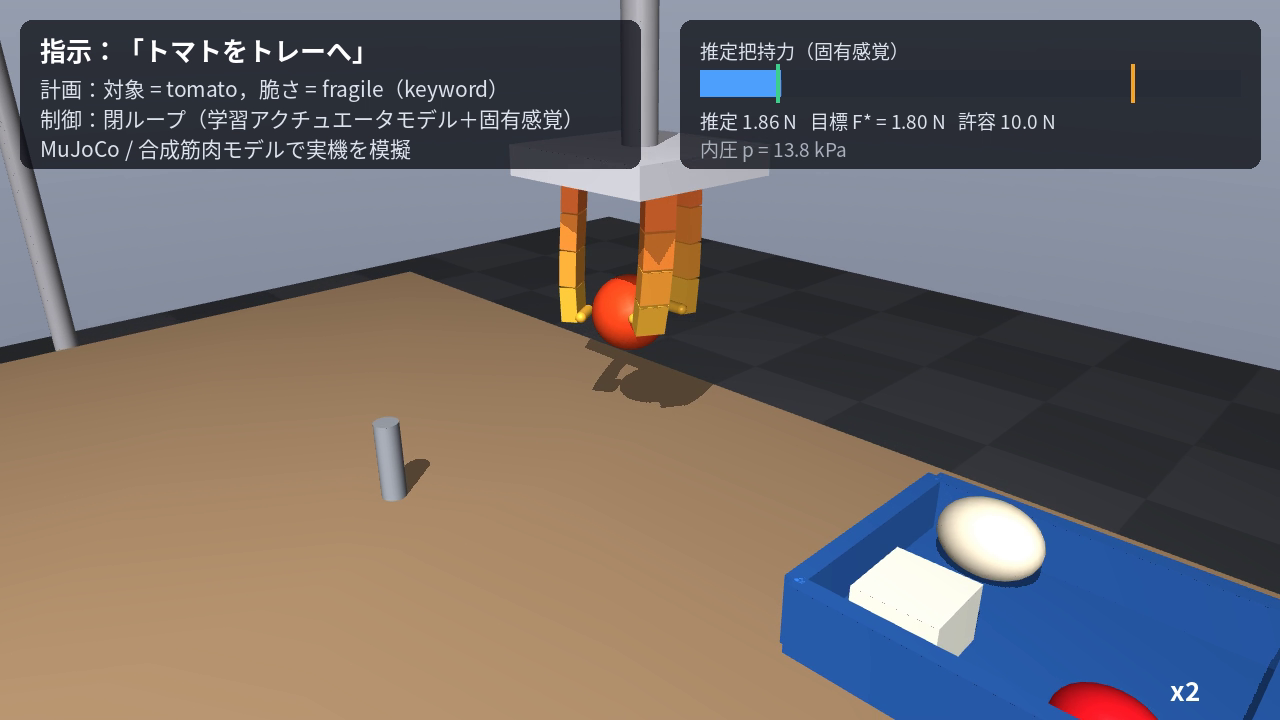
\includegraphics[width=\columnwidth]{frame_carry.png}
\caption{言語指示「トマトをトレーへ」で把持・搬送している様子（MuJoCo）．右上に推定把持力（青），目標 $F^*$（緑），許容力（橙）を表示．}
\label{fig:scene}
\end{figure}

\section{考察}
\textbf{なぜ学習モデルが効くのか．}固有感覚推定は「自由に曲がったらどこまで曲がるはずか」との差から力を求めるため，アクチュエータモデルの誤差がそのまま力の誤差になる．
同定で曲げ角誤差を下げることが，追加センサなしで 1\,N 以下の力を扱う前提条件だった．
\textbf{なぜ触覚が要るのか．}VLM は「何を，どれくらい優しく」の事前知識を言葉と画像から与えられるが，熟れ具合・中身・表面の滑りやすさはカメラに映らない．
SoftTwin では VLM を「最初の仮説」，固有感覚を「力の制御」，触覚スキンを「仮説の検証」と役割分担させた．弱く触ってから握り直す動作は，人が果物を手に取るときと同じである．
\textbf{産業上の意義．}物流・食品のピッキングでは，画像に比べて圧力や触覚のデータは集めにくく，ラベル付けもしにくい．
本手法の生成器は 1 試行約 0.7\,s で，画像と触覚・圧力・真の力・成否を同期したデータを量産できる．
家庭用ロボットでも，同じ見た目で状態の違う物（熟れた果物，中身の入った容器）を扱う場面は多い．
\textbf{RobOps．}評価は固定シードのクローズドループ成功率で行い，コード・データ・設定・学習済み重みを同じリポジトリで管理した．
\textbf{限界．}(i) 実機の代わりに合成筋肉モデルを用いた，(ii) 許容力は仮定値である，(iii) 定量評価の脆さクラスは指示文のキーワード解析で与え，VLM の精度は評価していない，(iv) Isaac Sim 版のセル（触覚の接触レポートも実装済み）との数値比較は未実施である，
(v) 物体の柔らかさは接触パラメータで近似しており有限要素の変形ではない，(vi) 触覚スキンの特性は仮定値で，実センサでの校正と sim-to-real 評価が必要である．

\section{まとめと今後}
学習アクチュエータモデルと固有感覚推定を組み合わせ，内圧固定では両立できない「潰さない」と「落とさない」をシミュレーション上で両立した．
さらに布状触覚スキンで「触って確かめてからつかむ」ことで，見た目では区別できない物体も扱えることを示し，そのための触覚付きデータを自動で量産する仕組みを作った．
今後はシリコーン人工筋肉と M5Stack による実機で同じ評価を行い，Isaac Sim のツインで実機との差 $e$ をリアルタイムに監視する．
コードは Apache-2.0，指の型などのハードウェア設計は CERN-OHL で公開する予定である．

\begin{table}[t]
\centering\small
\caption{講義内容との対応}
\begin{tabular}{@{}p{17mm}p{52mm}@{}}
\toprule
講義 & 本研究での対応 \\
\midrule
第1・2回 & 固定シードの閉ループ評価，設定と重みの版管理 \\
第3回 & 50\,Hz の制御周期，遅延の計測，時刻の扱い \\
第4・5回 & ROS~2 のトピック設計，記録→LeRobot 形式→学習 \\
第4・5回 & マルチモーダル（画像・触覚・圧力）データの自動生成と学習 \\
第6回 & OSS ライセンス，OSHW としての公開方針 \\
\bottomrule
\end{tabular}
\end{table}

\begin{thebibliography}{9}\small
\bibitem{shintake2018} J. Shintake, V. Cacucciolo, D. Floreano, H. Shea, ``Soft robotic grippers,'' \textit{Advanced Materials}, 30(29), 1707035, 2018.
\bibitem{ilievski2011} F. Ilievski, A. D. Mazzeo, R. F. Shepherd, X. Chen, G. M. Whitesides, ``Soft robotics for chemists,'' \textit{Angew. Chem. Int. Ed.}, 50(8), 1890--1895, 2011.
\bibitem{mosadegh2014} B. Mosadegh \textit{et al.}, ``Pneumatic networks for soft robotics that actuate rapidly,'' \textit{Adv. Funct. Mater.}, 24(15), 2163--2170, 2014.
\bibitem{howell2001} L. L. Howell, \textit{Compliant Mechanisms}, Wiley, 2001.
\bibitem{hwangbo2019} J. Hwangbo \textit{et al.}, ``Learning agile and dynamic motor skills for legged robots,'' \textit{Science Robotics}, 4(26), eaau5872, 2019.
\bibitem{todorov2012} E. Todorov, T. Erez, Y. Tassa, ``MuJoCo: A physics engine for model-based control,'' \textit{IROS}, 2012.
\bibitem{qwen25vl} S. Bai \textit{et al.}, ``Qwen2.5-VL technical report,'' arXiv:2502.13923, 2025.
\end{thebibliography}
\end{document}
